\subsection {Product Perspective}

In this paragraph we shall deepen the shared phenomena mentioned in the previous section, providing an oversight of the domain model on different levels of specification, by means of class and state diagrams.

\begin{itemize}

\item \textbf{Login (controlled by the world and observed by the machine)}: On every opening of the app, users must insert their phone number, then the code generated by the server and sent to them by SMS. Authorities enter using their ID code and password provided to them in a previous moment.

\item \textbf{File report (controlled by the world and observed by the machine)}: Users must take a photo of the violation and specify the type, position is obtained by the tracker in the phone, date and time are provided by the server, and a brief description can be attached. Nowithstanding that the system exploits convolutional neural network to identify the license plate of the vehicle in the photos, the user must add the number to improve the accuracy of the violation.In case of incomplete identification the user is warned and invited to retake the photo (violations with no photo or incomplete plate identification are not accepted, and the user must start over). If the violation complies with all this rules, it is sent to Safestreets' DBMS.

\item \textbf{Inspect violation (controlled by the world and observed by the machine)}: Authorities have access to all the pending violations of their city. They can discard the violation (its data is erased by the DBMS) or inspect it. Exploiting Google Maps' API, they are guided to the position of the violation. The result can be either positive (the violation is verified and a fine or a warning is issued) or negative. In the former option the violation is saved on the database, in the latter one, the data is discarded.

\item \textbf{Show data of violations (controlled by the machine and observed by the world)}: All the successful violations are stored on the DB with statistics regarding every street. Streets are ordered by the number of violations committed during the previous month in decreasing orderd. Users can select a street and acknowledge the number of violation type by type, authorities see also the list of the plates of the offenders.

\item \textbf{Show data of accidents (controlled by the machine and observed by the world)}: If the \\ municipality offers data about accidents it is crossed with that of Safestreets, street by street. Streets are ordered by the number of accidents, those who have a number of accidents equal to or greater than the treshold (for example \textcolor{Red}{\tres}) are marked unsafe, and the most common type of violation is shown. The number of accidents can be seen by everyone.

\item \textbf{Show suggestions (controlled by the machine and observed by the world)}: Suggestion are formulated for unsafe streets based on the most common type of violation, they can be seen only by the authorities.

\end{itemize}

Following are the class and state diagrams: \newpage

\begin{figure}[H]
\centering
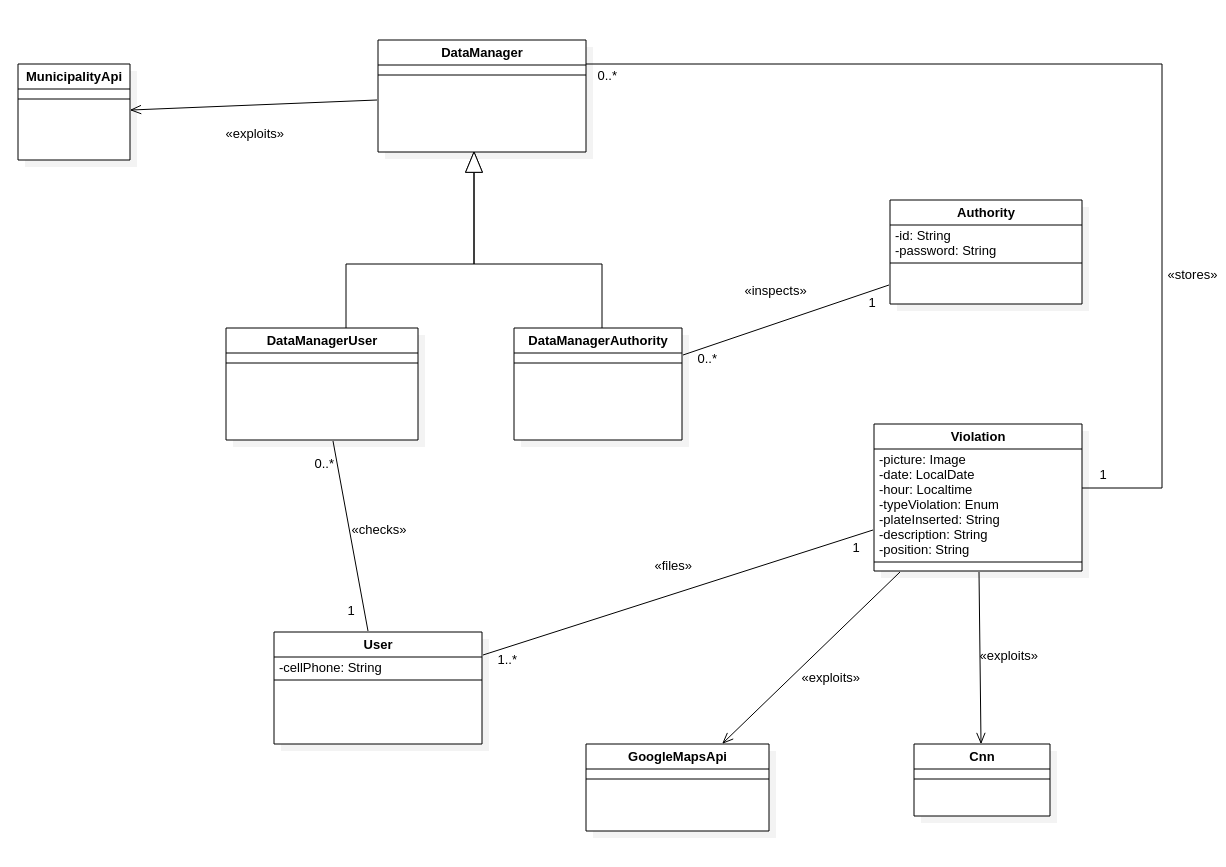
\includegraphics[width=\textwidth]{Images/Diagrams/uml.png}
\caption{\label{fig:UML}Class Diagram}
\medskip
\small
User and Authority are set as different objects as they undergo different kinds of authentication and have different levels of priviledges
\end{figure}

\begin{figure} [H]
\centering
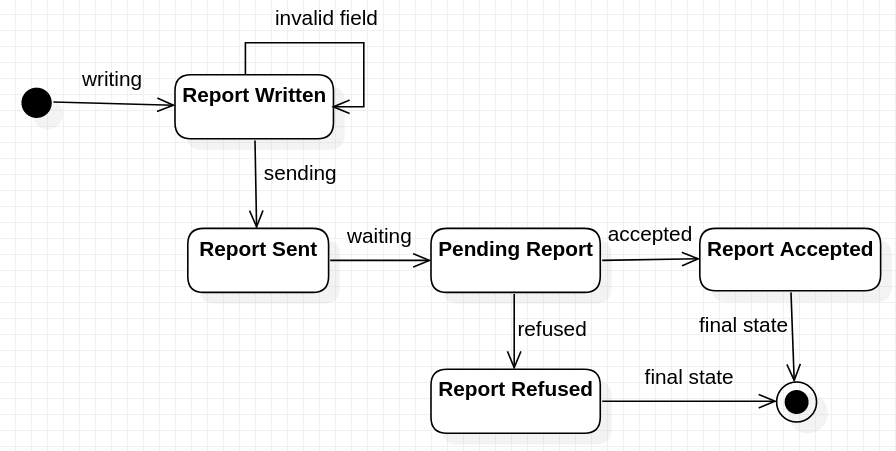
\includegraphics[width=\textwidth]{Images/Diagrams/State-1.png}
\caption{\label{fig:State-1}Statechart diagram for the basic function (user)}
\end{figure}

\begin{figure} [H]
\centering
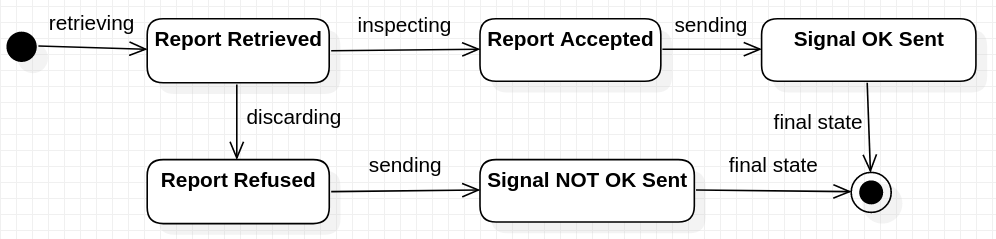
\includegraphics[width=\textwidth]{Images/Diagrams/State-2.png}
\caption{\label{fig:State-2}Statechart diagram for the basic function (authority)}
\end{figure}

\begin{figure} [H]
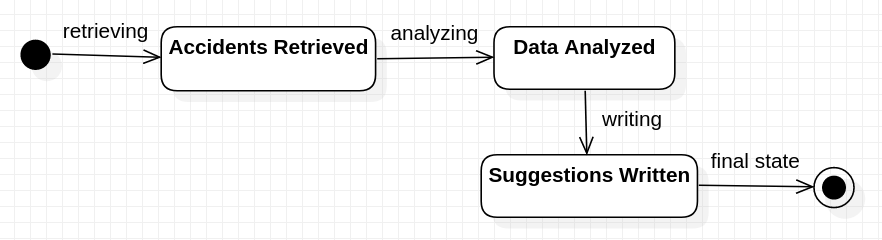
\includegraphics[width=\textwidth]{Images/Diagrams/State-3.png}
\caption{\label{fig:State-3}Statechart diagram for the advanced function}
\end{figure}

\subsection{Product Functions}

Here the most important features of the product are outlined:

\subsubsection{Data management}

Data offered by the municipality are replicated and not modified.

\subsubsection*{Data management by the users}

Users are allowed to send information about their violation on the DB but have no power over their conservation. 

\subsubsection*{Data management by the authorities}

Authorities have the power to delete (discard) a case, or to inspect it and close it, keeping it on the DB in the end. 

\subsubsection{Data Requests}

Users and authorities can retrieve information stored previously on the DB by the means of a DBMS.

\subsubsection*{Requests by the users}

Users are unable to see their previous report but can retrieve general information about violations under the form of a list of streets, ordered by the one with the greatest number of violation to the one with the smallest. Every street can be highlighted and the types of violations are ordered in a similar fashion. They can also access a list of streets with their respective number of accidents, ordered from the most unsafe street to the least unsafe one.

\subsubsection*{Requests by the authorities}

Authorities can access all the pending violations in their city. They have the same powers as the citizens but they can retrieve more info. When accessing the list of streets by violation, they are allowed to see the plates of repeated offenders of the street, from the most incorrect to the least. Upon inspection of the street, taken by the list which focuses on accidents, they are prompted with suggestions on how to improve the security of the street itself.


\subsection{Users characteristics}

\begin{itemize}

\item \textbf{User}: A citizen who has SafeStreets installed on their smartphone.

\item \textbf{Authority}: Social community workers or administrative workers who keep control of the in general,

\end{itemize}

\subsection{Assumptions, dependencies and constraints}

\subsubsection{Assumptions}

\subsubsection*{Basic Service}

\begin{itemize}

\item \textbf{D1}: The smartphone of the user can provide accurate location

\item \textbf{D2}: The data provided by the user is correct

\item \textbf{D3}: Internet connection is reliable

\item \textbf{D4}: The CNN is always on and ready to communicate

\item \textbf{D5}: There is no failure in communication

\item \textbf{D6}: GM is always on and ready to communicate

\item \textbf{D7}: Data storage is reliable

\end{itemize}

\subsubsection*{Advanced Funcionality}

\begin{itemize}

\item \textbf{D8}: Data offered by municipality is correct

\item \textbf{D9}: Data offered by municipality is up-to-date

\end{itemize}

\subsubsection{Dependencies}

\begin{itemize}

\item The system needs a DBMS to store and retrieve data

\item GM is provided by Google

\item CNN is provided by an external body

\end{itemize}

\subsubsection{Constraints}

\begin{itemize}

\item Users must be equipped with smartphones provided with camera, internet connection and GPS tracker

\item Authorities must be equipped with smartphones provided with camera, internet connection and GPS tracker or a computer with a working internet connection and a browser installed upon.

\item Users' smartphone mount an OS compatible with the application

\item Authorities' smartphone mount an OS compatible with the application

\item Authorities' computer has an internet browser installed upon

\end{itemize}